\documentclass{amsart}

% biber

\usepackage[english]{babel}
\usepackage[utf8]{inputenc}
\usepackage{graphicx}
\usepackage{mathtools}
\usepackage{amsthm}
\usepackage{thmtools,thm-restate}
\usepackage{amsfonts}
\usepackage{hyperref}
\usepackage[backend=biber,url=true,doi=true,eprint=false,style=alphabetic]{biblatex}
\usepackage{enumitem}
\usepackage[justification=centering,singlelinecheck=false]{caption}
\usepackage{indentfirst}
\usepackage{algorithm}
\usepackage{algpseudocode}
\usepackage{listings}
\usepackage[x11names, rgb]{xcolor}
\usepackage{tikz}
\usepackage{hyperref}
\usepackage{subcaption}
\usepackage{booktabs}
\usepackage{linegoal}
\usepackage{csquotes}
\usetikzlibrary{snakes,arrows,shapes}

\addbibresource{references.bib}

\makeatletter
\def\subsection{\@startsection{subsection}{3}%
  \z@{.5\linespacing\@plus.7\linespacing}{.1\linespacing}%
  {\normalfont}}
\makeatother

\makeatletter
\patchcmd{\@setauthors}{\MakeUppercase}{}{}{}
\makeatother

\DeclareMathOperator*{\argmin}{arg\,min}
\DeclareMathOperator*{\argmax}{arg\,max}
\DeclareMathOperator*{\Val}{\text{Val}}
\DeclareMathOperator*{\Ch}{\text{Ch}}
\DeclareMathOperator*{\Pa}{\text{Pa}}
\DeclareMathOperator*{\Sc}{\text{Sc}}
\newcommand{\ov}{\overline}
\newcommand{\region}{\mathcal}

\newcommand\defeq{\mathrel{\overset{\makebox[0pt]{\mbox{\normalfont\tiny\sffamily def}}}{=}}}

\newcommand{\algorithmautorefname}{Algorithm}
\algrenewcommand\algorithmicrequire{\textbf{Input}}
\algrenewcommand\algorithmicensure{\textbf{Output}}
\algnewcommand{\LineComment}[1]{\State\,\(\triangleright\) #1}

\captionsetup[table]{labelsep=space}

\theoremstyle{plain}

\newcounter{dummy-def}\numberwithin{dummy-def}{section}
\newtheorem{definition}[dummy-def]{Definition}
\newcounter{dummy-thm}\numberwithin{dummy-thm}{section}
\newtheorem{theorem}[dummy-thm]{Theorem}
\newcounter{dummy-prop}\numberwithin{dummy-prop}{section}
\newtheorem{proposition}[dummy-prop]{Proposition}
\newcounter{dummy-corollary}\numberwithin{dummy-corollary}{section}
\newtheorem{corollary}[dummy-corollary]{Corollary}
\newcounter{dummy-lemma}\numberwithin{dummy-lemma}{section}
\newtheorem{lemma}[dummy-lemma]{Lemma}
\newcounter{dummy-ex}\numberwithin{dummy-ex}{section}
\newtheorem{exercise}[dummy-ex]{Exercise}
\newcounter{dummy-eg}\numberwithin{dummy-eg}{section}
\newtheorem{example}[dummy-eg]{Example}

\numberwithin{equation}{section}

\newcommand{\set}[1]{\mathbf{#1}}
\newcommand{\pr}{\mathbb{P}}
\newcommand{\eps}{\varepsilon}
\renewcommand{\implies}{\Rightarrow}

\newcommand{\bigo}{\mathcal{O}}

\setlength{\parskip}{1em}

\lstset{frameround=fttt,
	numbers=left,
	breaklines=true,
	keywordstyle=\bfseries,
	basicstyle=\ttfamily,
}

\newcommand{\code}[1]{\lstinline[mathescape=true]{#1}}
\newcommand{\mcode}[1]{\lstinline[mathescape]!#1!}
\newcommand{\dset}[1]{\mathcal{#1}}

\title{%
  \noindent\rule{13cm}{1.0pt}\\
  \vspace{0.2cm}
  The Poon-Domingos Parameter Learning Algorithm for Image Completion and Classification on
  Sum-Product Networks
  \noindent\rule{13cm}{0.8pt}
}
\xdef\shorttitle{The Poon-Domingos Algorithm}
\author[]{\normalsize\textbf{Renato Lui Geh}\\\small Computer Science\\Institute of Mathematics
  and Statistics\\University of São Paulo\\\texttt{renatolg@ime.usp.br}}

\begin{document}

\begin{abstract}
  In this document we describe the Poon-Domingos~\cite{poon-domingos} parameter learning algorithm
  for image classification and completion.
  \vspace*{-3.5em}
\end{abstract}

\maketitle

\section{Structure}

The Poon-Domingos algorithm uses a fixed structure and then learns the weights through generative
learning. We first give an overview on how to build the structure given an image and then provide a
pseudo-code algorithm for building such structure. In this document we assume instances as images.
However, the Poon-Domingos structure allows for any object with local dependencies.

\subsection{Overview}

The Poon-Domingos structure models a probability distribution over a set of variables with local
dependencies. On the plain, one could argue it models rectangular neighborhoods for each point in
the space. In the article~\cite{poon-domingos}, Poon and Domingos use images as a dataset, with
dependencies being rectangular pixel neighborhoods. Images are an example of local dependencies,
since a pixel has possible dependencies with their neighbors.

Dennis and Ventura explain an intuition of how the Poon-Domingos structure algorithm
works~\cite{clustering}. We expand on this intuition, giving insights on how such an algorithm is
built and showing a pseudo-code visualization of it. Once we have shown how to build the SPN
structure, we describe generative learning through gradient descent, and later
expectation-maximization.

\begin{figure}[h]
  \centering
  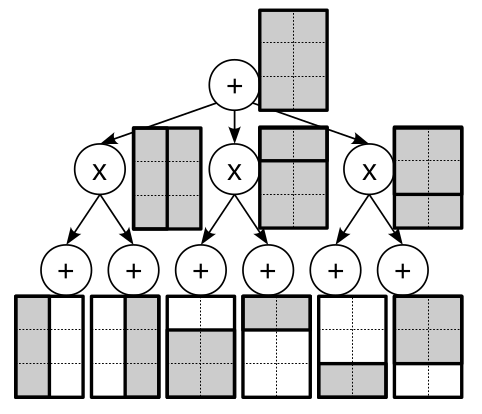
\includegraphics[scale=1.0]{imgs/dv_spn.png}
  \captionsetup{justification=raggedright}
  \caption{The Poon architecture with $r=1$ resolution and $k=1$ sum nodes per region on a
  2$\times$3 image. At each $r$ resolution axis-aligned rectangular decomposition, we create $k$
  sum nodes.\cite{clustering}\label{fig:dv_spn}}
\end{figure}

\subsection{Definitions and properties}

\begin{definition}[Region]
  A Region $\region{R}$ is a rectangular part of an image. Let $p_0=(x_0, y_0)$ and $p_1=(x_1,
  y_1)$ be the top-left and bottom-right pixels of $\region{R}$ relative to the image. These are
  called the coordinates of $\region{R}$.
\end{definition}

\begin{definition}[Region Node]
  A Region Node $R$ has a one-to-one and onto mapping with a Region $\region{R}$. $R$ has $k$
  internal nodes associated with it. If $\region{R}$ is over an $r\times r$ set of pixels (i.e.\
  the atomic unit), then $R$ has $k$ leaf nodes (e.g.\ $k$-mixture of gaussians). Else, $R$ has $k$
  sum nodes.
\end{definition}

\begin{definition}[Decomposition]
  Let $\region{R}$ be a Region. A Decomposition $\mathcal{D}$ is an axis-aligned partitioning of
  $\region{R}$ into two Regions $\region{R}_1$ and $\region{R}_2$.
\end{definition}

The decomposition $\mathcal{D}$ of a Region $\region{R}$ involves a few steps. Let $\region{R}_1$
and $\region{R}_2$ be the resulting subregions product of the decomposition. The resulting subgraph
of the SPN $S$ of this decomposition is a DAG $G$. If $\region{R}$ is the entire image, then the
root of $G$ is a single sum node and $G=S$. Otherwise, then the root of $G$ is a region node and
thus the root of $G$ is a set of $k$ sum nodes. Let $R$ be the root node of $G$. Region nodes $R_1$
and $R_2$ will both have $k$ sum nodes (or univariate distributions for leaves). We shall denote as
$R_i^j$ the $j$-th sum node of region node $i$. For each pairing of sum nodes $(R_1^i, R_2^j)$, we
create a product node $\pi$ and add $R_1^i$ and $R_2^j$ as children of $\pi$. The set $\Pi$ of
these product nodes are the decomposition nodes of $\region{R}$ into $\region{R}_1$ and
$\region{R}_2$.  Once we have created all product nodes in this set, we add all of them as children
of $R$. If $R$ is a region node, then adding $\Pi$ as children of $R$ means, for every sum node
$\sigma$ in $R$, set product node $\pi\in\Pi$ as a child of $\sigma$. Each product set $\Pi$ will
have $\binom{m}{2}$ product nodes, since we take every distinct pairing of sum nodes in $R_1$ and
$R_2$.

\begin{figure}[h]
  \centering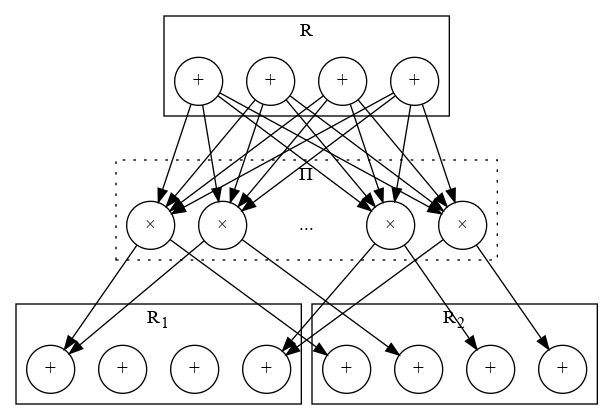
\includegraphics[scale=0.4]{graphs/decomp.png}
  \caption{A decomposition of a Region $\region{R}$ into two subregions $\region{R}_1$ and
  $\region{R}_2$. The set $\Pi$ of product nodes are the decomposition nodes that connect the
  unsplit image to the partitions. Each element $\pi\in\Pi$ connects a pairing of a sum node of
  $\region{R}_1$ and of $\region{R}_2$.\label{fig:decomp}}
\end{figure}

Since a region node $R$ is unique, we may have different decompositions in which the same region
appears more than once. For this reason we should create a single Region Node for each possible
region. We need a map function that takes the top-left and bottom-right pixel positions of a region
and maps it to a number for storage. Since every region is unique, we need a one-to-one and onto
function.

\begin{definition}[Region map function]
  A region map function is a function that maps a region into an integer. We define it as
  \begin{align*}
    &f:\mathbb{Z}_m\times\mathbb{Z}_n\times\mathbb{Z}_m\times\mathbb{Z}_n\to\mathbb{Z}_{m^2n^2}\\
    &f(x_1, y_1, x_2, y_2) = ((y_1m+x_1)m+x_2)n+y_2
  \end{align*}
  where $x_1,x_2\in\mathbb{Z}_m$ and $y_1,y_2\in\mathbb{Z}_n$.
\end{definition}

\begin{proposition}
  The region map function is one-to-one and onto.
\end{proposition}
\begin{proof}
  We first prove $f$ is one-to-one. If $f$ is injective, then $f(x_1,y_1,x_2,y_2) =
  f(x_1',y_1',x_2',y_2') \implies (x_1,y_1,x_2,y_2)=(x_1',y_1',x_2',y_2')$. Suppose
  $f(x_1,y_1,x_2,y_2)=f(x_1',y_1',x_2',y_2')$ for some $x_i\in\mathbb{Z}_m$ and
  $y_i\in\mathbb{Z}_n$. Then we have:
  \begin{align*}
    &((y_1m+x_1)m+x_2)n+y_2=((y_1'm+x_1')m+x_2')n+y_2'\\
    &(m^2y_1+mx_1+x_2)n+y_2=(m^2y_1'+mx_1'+x_2')n+y_2'\\
    &m^2ny_1+mnx_1+nx_2+y_2=m^2ny_1'+mnx_1'+nx_2'+y_2'\\
    &m^2n(y_1-y_1')+mn(x_1-x_1')+n(x_2-x_2')+(y_2-y_2')=0
  \end{align*}
  But $m,n>0$. Therefore, it is easy to see that $x_i-x_i'=0$ and $y_i-y_i'=0$ is necessary for the
  equation to hold. Proof of surjection is simple. Since we know $f$ is one-to-one and that
  $\mathbb{Z}_m\times\mathbb{Z}_n\times\mathbb{Z}_m\times\mathbb{Z}_n$ has the same number of
  elements as $\mathbb{Z}_{m^2n^2}$, than it follows that $f$ must be onto.
\end{proof}

Bijection of the region map function is necessary since we need the inverse function $f^{-1}$ to be
symmetrical to $f$. That is, we must be able to encode a region into a number and later be able to
find what region a number represents. We define the inverse function of $f$ below.

\begin{definition}[Inverse region map function]
  The inverse of the region map function is given by the decomposition of an integer
  $r\in\mathbb{Z}_{m^2n^2}$ into a tuple $(x_1,y_1,x_2,y_2)\in\mathbb{Z}_m\times\mathbb{Z}_n\times
  \mathbb{Z}_m\mathbb{Z}_n$. Let $g=f^{-1}$. We define $g$ as an algorithm as follows
  \begin{algorithm}[H]
    \caption{\normalfont{Function \code{Encode} $\coloneqq f^{-1} = g$}}
    \begin{algorithmic}[1]
      \normalfont%
      \Require\,$r\in\mathbb{Z}_{m^2n^2}$
      \Ensure\,$(x_1,y_1,x_2,y_2)\in\mathbb{Z}_m\times\mathbb{Z}_n\times\mathbb{Z}_m\times\mathbb{Z}_n$
      \State\,$y_2\gets i \mod n$
      \State\,Let $c\in\mathbb{Z}_{m^2n^2}$
      \State\,$c\gets\frac{(r-y_2)}{n}$
      \State\,$x_2\gets c \mod m$
      \State\,$c\gets\frac{c-x_2}{m}$
      \State\,$x_1\gets c \mod m$
      \State\,$y_1\gets\frac{c-x_1}{w}$
      \State\,\textbf{return} $(x_1,y_1,x_2,y_2)$
    \end{algorithmic}
  \end{algorithm}
\end{definition}

\subsection{Structural algorithm}

We now show how to construct the Poon-Domingos architecture given an image $I$ (which is equivalent
to a Region consisting of the entire image), resolution $r$ and $m$ sum nodes per region.

The algorithm, as summarized in the last subsection, can be constructed recursively. However we
avoid this technique in favor of an iterative version, which uses less memory. We must first do a
preprocessing of Regions. We iterate over all possible subrectangles in $I$, create a Region for
each of them and assign an identification number to it. This number is the value of the region map
function given the region's position. We name the region map function as \code{Encode} that takes a
region position and returns a non-negative integer. Similarly, we name the inverse function of
\code{Encode} as \code{Decode} that takes a non-negative integer and returns a region position.

We denote by $[\region{R}]$, where $\region{R}$ is a region, a function that returns a pair of
positive integers that represent the width and height of $\region{R}$. Once we have constructed all
possible regions, we iterate over all possible decompositions according to the following steps:

\begin{enumerate}[label=\arabic*.]
  \item\label{start-label} Select each possible region $\region{R}$ in image $I$
  \item If $\region{R} = I$, then $R$ is a sum node and is root
  \item Else if $R$ contains only gaussians, skip this region
  \item Else, $R$ exists and is a set of sum nodes
  \item Partition $\region{R}$ into a pairing of subregions $\region{R}_1$ and $\region{R}_2$
  \item For each subregion $\region{R}_i$
    \begin{enumerate}[label*=\arabic*]
      \item Let $(w, h) \gets \region{R}_i$
      \item If $w > r$ and $h > r$ then region node $R_i$ must be a set of $m$ gaussians
      \item Else, region node $R_i$ must be a set of $m$ sum nodes
    \end{enumerate}
  \item Create a set $\Pi$ of product nodes
  \item For each pair $(R_1^i, R_2^j)$, where $R_p^q$ is the inner node $q$ of subregion node $R_p$
    \begin{enumerate}[label*=\arabic*]
      \item Create a product node $\pi$ and add it to set $\Pi$
      \item Add $R_1^i$ and $R_2^j$ as children of $\pi$
      \item Add $\pi$ as child of all inner sum nodes of $R$
    \end{enumerate}
  \item Go to step~\ref{start-label}
\end{enumerate}

\begin{algorithm}[H]
  \caption{\code{CreateRegions}}\label{alg:createregions}
  \begin{algorithmic}[1]
    \Require\,A pair $(w,h)$ representing the image $I$ dimensions
    \Require\,Dataset $\mathcal{D}$
    \Require\,Integer $m$ as number of components in each Region
    \Require\,Integer $r$ as resolution
    \Ensure\,A list $\mathcal{L}$ of Nodes indexed by their region map function value
    \State\,Let $n=w\cdot h$
    \For{$i\gets 0..(n-1)$}
      \State\,$x_1\gets i\mod w$
      \State\,$y_1\gets i/w$
      \For{$x_2\gets (w-1)..x_1$ decreasingly}
        \For{$y_2\gets (h-1)..y_1$ decreasingly}
          \If{$x_1=0$ and $y_1=0$ and $x_2=w-1$ and $y_2=h-1$}
            \LineComment{The entire image is the root sum node}
            \State\,$j\gets$\mcode{Encode$(x_1,y_1,x_2,y_2)$}
            \State\,$\mathcal{L}[j]\gets$\mcode{SumNode$()$}
            \LineComment{\code{SumNode} returns a sum node}
          \EndIf%
          \State\,Let $R$ be a new Region node\label{alg:createregions-mk1}
          \State\,Let $d_x=x_2-x_1$ and $d_y=y_2-y_1$
          \If{$d_x < r$ or $d_y < r$}
            \State\,$x\gets\max(x_1+r,x_2)$
            \State\,$y\gets\max(y_1+r,y_2)$
            \State\,$r\gets$\mcode{Encode$(x_1,y_1,x,y)$}
            \State\,$R\gets\mathcal{L}[r]$\label{alg:createregions-mk2}
          \ElsIf{$d_x = r$ and $d_y = r$}
            \State\,$R\gets$\mcode{GaussianMixture$(x_1, y_1, x_2, y_2, D, m)$}
            \LineComment{\code{GaussianMixture} returns a node containing $m$ gaussians}
          \Else%
            \State\,$R\gets$\mcode{RegionNode$(m)$}
            \LineComment{\code{RegionNode} returns a node containing $m$ sum nodes}
          \EndIf%
          \State\,$j\gets$\mcode{Encode$(x_1,y_1,x_2,y_2)$}
          \State\,$\mathcal{L}[j]\gets R$
        \EndFor%
      \EndFor%
    \EndFor%
    \State\,\textbf{return} $\mathcal{L}$
  \end{algorithmic}
\end{algorithm}

The structural algorithm is almost complete. The main object of interest now is on finding all
possible regions in an image. Consider the matrix $M_{n\times m}$ as the image representation of
$I$ indexed by 0. Then we can find all possible regions by iteration over every top-left position
$(x,y)$ and for each of these positions iterating over all bottom-right pixels $(x+p,y+q), 0\leq
p<n, 0\leq q<m$.

We assume a dataset $\mathcal{D}$ where each instance $\mathcal{D}[X]$ gives an ordered sequence of
integers corresponding to the image pixels in expanded form. Let $R$ be a region, $(x_1,y_1)$ be
its top-left position and $(x_2,y_2)$ its bottom-right position. We call $(x_1,y_1,x_2,y_2)$ the
coordinates of $R$.

\begin{proposition} Let $R_1$ be the region in Line~\ref{alg:createregions-mk1}.
  Line~\ref{alg:createregions-mk2} in function \code{CreateRegions} always yields
  a region $R_2$ that has already been previously created.
\end{proposition}
\begin{proof}
  Let $(x_1,y_1)$ be $R_1$'s top-left position. We fix $x_2\geq x_1+r$. The third \code{for} loop
  in \code{CreateRegions} yields a decreasing sequence from $h-1$ to $y_1$. So for each $y_2$ in
  this ordered sequence, the previous instance will have already been computed. It then follows
  that for every $y_2=y_1+r-k$, $0\leq k\leq r$, it is true that $y_1+r$ has already been computed.
  We do the same for $x_2$ by fixing $y_2\geq y_1+r$. When both $x_2<x_1+r$ and $y_2<y_1+r$, we
  fall into the previous subcases.
\end{proof}

\begin{algorithm}[h]
  \caption{\code{Structure}}\label{alg:structure}
  \begin{algorithmic}[1]
    \Require\,A pair $(w,h)$ representing the image $I$ dimensions
    \Require\,Dataset $\mathcal{D}$
    \Require\,Integer $m$ as number of components in each Region
    \Require\,Integer $r$ as resolution
    \Ensure\,An SPN $S$ containing the learned structure from image $I$
    \State\,$\mathcal{L}\gets$\mcode{CreateRegions$(w, h, D, m, r)$}
    \State\,$s\gets$\mcode{Encode$(0,0,w-1,h-1)$}
    \State\,$S\gets\mathcal{L}[s]$
    \LineComment{$S$ is the root node}
    \For{each key and value pair $(k,R)$ in $\mathcal{L}$}
      \If{$k = s$}
        \State\,\textbf{skip}
      \EndIf%
      \State\,$(x_1,y_1,x_2,y_2)\gets$ \mcode{Decode$(k)$}
      \State\,\mcode{LeftQuadrant$(x_1,y_1,x_2,y_2,\mathcal{L})$}
      \State\,\mcode{BottomQuadrant$(x_1,y_1,x_2,y_2,\mathcal{L})$}
    \EndFor%
    \State\,\textbf{return} $S$
  \end{algorithmic}
\end{algorithm}

Next, we clarify functions \mcode{LeftQuadrant} and \mcode{BottomQuadrant}. Recall the algorithm
outline we listed earlier. For each decomposition of a region into two subregions, we must create a
set of product nodes whose internal products nodes are connected the two distinct subregion
internal nodes. Let $R$ be a region. Our goal is to find the parent regions of $R$. In other words,
we must find all possible decompositions in which $R$ is one of the two disjoint subregions. Since
we only take axis-aligned decompositions into account, we can represent all possible decompositions
of $R$ as tightly-bound subrectangles.

\begin{figure}[h]
  \centering
  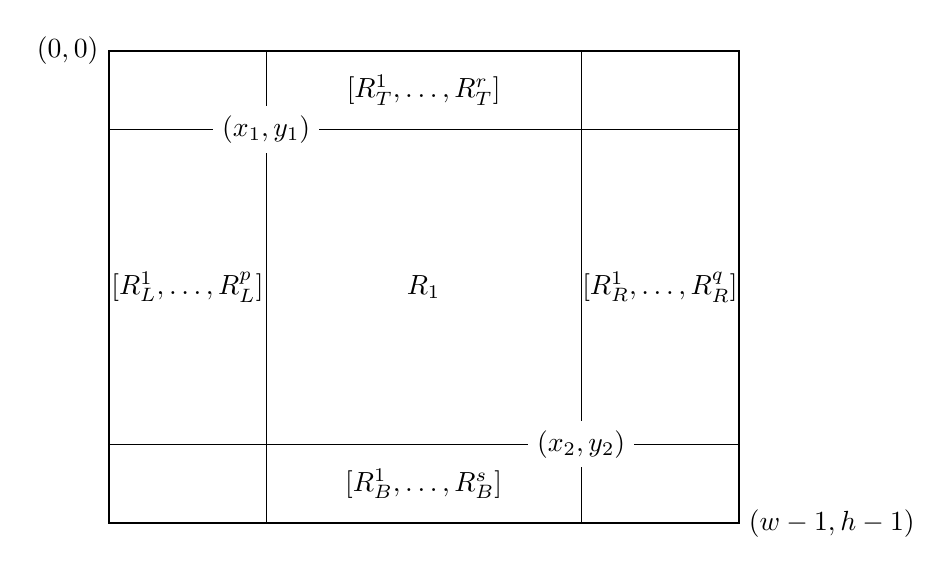
\begin{tikzpicture}
    \draw[thick] (0,0)
      -- (8, 0) node[right,fill=white] {$(w-1,h-1)$}
      -- (8, 6)
      -- (0, 6) node[left,fill=white] {$(0,0)$}
      -- cycle;
    \draw (2,0) -- (2,5) -- (6,5) -- (6,0) -- cycle;
    \draw (0,5) -- (6,5) -- (6,1) -- (0,1) -- cycle;
    \draw (2,6) -- (2,1) -- (6,1) -- (6,6) -- cycle;
    \draw (8,1) -- (2,1) -- (2,5) -- (8,5) -- cycle;
    \draw (4,3) node {$R_1$};
    \draw (1,3) node {$[R_L^1,\ldots,R_L^p]$};
    \draw (7,3) node {$[R_R^1,\ldots,R_R^q]$};
    \draw (4,5.5) node {$[R_T^1,\ldots,R_T^r]$};
    \draw (4,0.5) node {$[R_B^1,\ldots,R_B^s]$};
    \draw (2,5) node[fill=white] {$(x_1,y_1)$};
    \draw (6,1) node[fill=white] {$(x_2,y_2)$};
  \end{tikzpicture}
  \captionsetup{justification=raggedright}
  \caption{Given a decomposition of a region into two subregions, where one of them is $R_1$, we
  can find any possible complementary regions of $R_1$ by searching each quadrant. The image above
  shows all possible decompositions containing $R_1$, where the set $[R_Q^1,\ldots,R_Q^m]$, where
  $Q$ is a quadrant, contains all complementary regions of $R_1$ in the direction of $Q$. A
  decompositon is two regions $R_1$ and $R_Q^i$.}
\end{figure}

To find all the decompositions that contains a region $R_1$, we take each possible quadrant (we
name them $\{L,R,T,B\}$ for Left, Right, Top and Bottom) and then take all possible $R_Q^i$ region,
where $Q$ is the quadrant and $i$ the $i$-th region in $Q$. It suffices to find decompositions from
$L$ and $B$, as we will eventually do the same for the complementary region of $R_1$, which will
account for the $R$ and $T$ quadrants.

\begin{figure}[h]
  \centering
  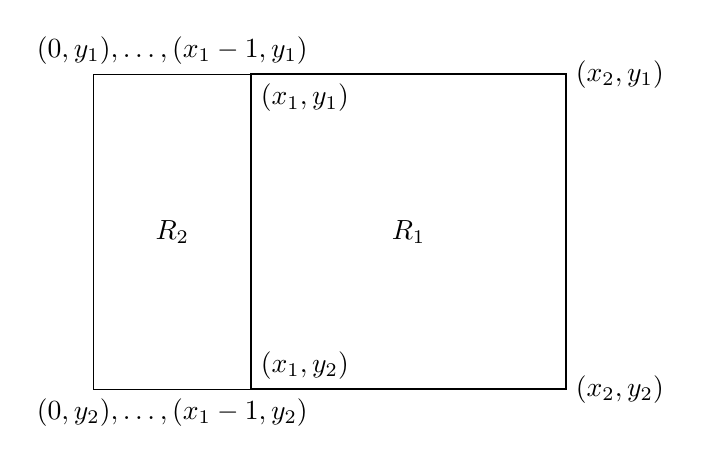
\begin{tikzpicture}
    \draw (0,0) -- (0,4) -- (2,4) -- (2,0) -- cycle;
    \draw[thick] (2,0) -- (2,4) -- (6,4) -- (6,0) -- cycle;
    \draw (1,2) node {$R_2$};
    \draw (4,2) node {$R_1$};
    \draw (1,0) node[anchor=north] {$(0,y_2),\ldots,(x_1-1,y_2)$};
    \draw (1,4) node[anchor=south] {$(0,y_1),\ldots,(x_1-1,y_1)$};
    \draw (2,4) node[anchor=north west] {$(x_1,y_1)$};
    \draw (2,0) node[anchor=south west] {$(x_1,y_2)$};
    \draw (6,4) node[right] {$(x_2,y_1)$};
    \draw (6,0) node[right] {$(x_2,y_2)$};
  \end{tikzpicture}
  \captionsetup{justification=raggedright}
  \caption{The left quadrant. Region $R_2$ is the complementary region of $R_1$ and can take any
  coordinates $(x',y_1,x_1,y_2)$, where $0\leq x'\leq x_1-1$.\label{fig:left-quadrant}}
\end{figure}

\autoref{fig:left-quadrant} shows a decomposition that contains subregions $R_1$ and $R_2$. Let
$(x_1,y_1,x_2,y_2)$ be the coordinates to $R_1$. We have $x_1$ subregions $R_2$ that are possible
decompositions with $R_1$. Similarly for~\autoref{fig:bottom-quadrant}, we have $y_1$ possible
subregions $R_2$. Consider the left quadrant. If $R_1$ switches place with $R_2$, it becomes clear
that we now have the right quadrant. Similarly for the bottom quadrant, by switching $R_1$ and
$R_2$, we have the top quadrant. This means our previous assumption that it is enough to take the
left and bottom quadrant is correct.

\begin{figure}[h]
  \centering
  \begin{tikzpicture}
    \draw (0,0) -- (0,5) -- (4,5) -- (4,0) -- cycle;
    \draw[thick] (0,0) -- (0,4) -- (4,4) -- (4,0) -- cycle;
    \draw (2,4.5) node {$R_2$};
    \draw (2,2) node {$R_1$};
    \draw (0,0) node[left] {$(x_1,y_2)$};
    \draw (4,0) node[right] {$(x_2,y_2)$};
    \draw (0,4) node[anchor=north west] {$(x_1,y_1)$};
    \draw (4,4) node[anchor=north east] {$(x_2,y_1)$};
    \draw (0,4.5) node[left] {$(x_1,0),\ldots,(x_1,y_1-1)$};
    \draw (4,4.5) node[right] {$(x_2,0),\ldots,(x_2,y_1-1)$};
  \end{tikzpicture}
  \captionsetup{justification=raggedright}
  \caption{The left bottom. Region $R_2$ is the complementary region of $R_1$ and can take any
  coordinates $(x_1,y',x_2,y_1)$, where $0\leq y'\leq y_1-1$.\label{fig:bottom-quadrant}}
\end{figure}

At each pairing of subregions $R_1$ and $R_2$ in a quadrant $Q$, we must create a set of product
nodes $\Pi$.

%--------------------------------------------------------------------------------------------------

\printbibliography[]

\end{document}
